% Drawing 69/05-8 -- folder 69, batch 05, archive page 86 (PDF page 87).
% Transcription: À gauche, une étoile marquée $A$, et au-dessus $\mathbb{F}_2^{\,i}$ \uncertain{} et un trait vertical.
% Kind: star of edges marked A. Method 2 (schematic redraw from the facsimile). Status: ok.
% Notes: The 'star' marked A: three centres joined in a triangle, each carrying four narrow spikes, each spike two strokes from its centre, closed at the tip or not as on the page: at the top centre a long vertical spike (its right stroke heavy) and three spikes from a point just above the centre, to the upper right, the right and (the lowest, from the centre's right) to the right; at the left centre a long spike to the left and three downwards, the last from a heavy dot just under the centre; at the right centre one to the right (a heavy dot at its tip), one down to the right and two downwards. Above it F_2^i (uncertain, as in the transcription) and a short vertical stroke. Not drawn: a small blot under the left side of the triangle and a small ring beside the right lower spikes (marks, not read). Redrawn 2026-11-09 (issue 128). Overlay check 2026-11-13 (claude-opus-5-5, issue 147): the 300 dpi colour rendering of the 250 ppi scan laid under the redraw, rasterised from its TikZ (not compiled: no TeX in the session). The three centres were 1 to 2 units off and the spikes had been drawn as twelve closed triangles of a standard shape, several 2 to 4 units off their ink; every spike is now drawn stroke by stroke on its ink, the top spikes from the point where they gather on the page, the open and closed tips as they are. Matches the facsimile.
% Coordinates: 1 unit = 1 mm = 1/100 of the crop width (bbox in page fractions: [0.1, 0.47, 0.32, 0.6]).
% Redrawn by Claude (claude-opus-5-5), issue #73, 2026-11-09; not checked by a human; not compiled (no TeX in the session).
% Checked by Claude (claude-opus-5-5) 2026-11-13 (issue #147): overlaid on the colour scan (250 ppi, rendered at 300 dpi) and corrected; not compiled (no TeX in the session), rasterised for the overlay by a Python reader of this TikZ. Status: ok.
% Rights: reproduces part of the work -- behind RENDER_TRANSCRIPTS, never published by itself.
\documentclass[tikz,border=3pt]{standalone}
\usepackage{amsmath,amssymb}
\usetikzlibrary{patterns,arrows.meta}
\tikzset{pencil/.style={black!45}, struck/.style={black!35}, mark/.style={circle,draw,inner sep=1.3pt}, pt/.style={circle,fill,inner sep=0.9pt}, opt/.style={circle,draw,fill=white,inner sep=1.1pt}}
\begin{document}
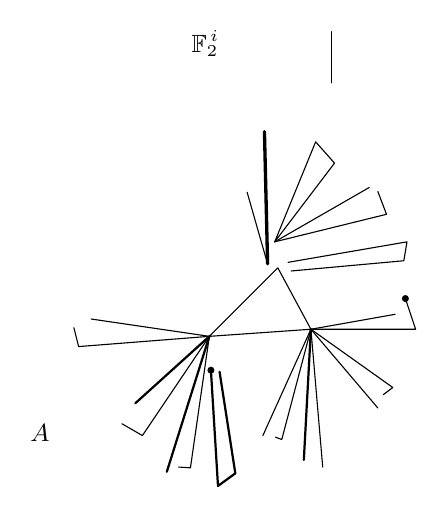
\begin{tikzpicture}[x=1mm,y=1mm,line cap=round,line join=round,font=\scriptsize]
\draw (61.2,-36.5) -- (52.5,-45.2) -- (65.4,-44.3) -- cycle;
\draw[very thick] (59.9,-36) -- (59.5,-19.2);
\draw (59.9,-36) -- (57.3,-26.9);
\draw (60.8,-33.2) -- (66,-20.5) -- (68.4,-23.2) -- cycle;
\draw (60.8,-33.2) -- (72.8,-26.3);
\draw (60.8,-33.2) -- (75,-29.7) -- (73.9,-26.8);
\draw (62.5,-35.8) -- (77.6,-33.2) -- (77.2,-35.6) -- (62.9,-36.9);
\draw (52.5,-45.2) -- (37.5,-43);
\draw (52.5,-45.2) -- (35.9,-46.5) -- (35.3,-44.1);
\draw[thick] (52.5,-45.2) -- (43.1,-53.7);
\draw (52.5,-45.2) -- (44,-57.8) -- (41.4,-56.3);
\draw[thick] (52.5,-45.2) -- (47.1,-62.4);
\draw (52.5,-45.2) -- (50.1,-61.9) -- (48.6,-61.8);
\draw[thick] (52.7,-49.5) -- (53.6,-64.2) -- (55.8,-62.6) -- (53.8,-49.7);
\node[pt] at (52.7,-49.5) {};
\draw (65.4,-44.3) -- (76.1,-42.4);
\draw (65.4,-44.3) -- (78.7,-44.3) -- (77.4,-40.4);
\node[pt] at (77.4,-40.4) {};
\draw (65.4,-44.3) -- (75.8,-51.7) -- (74.6,-52.6);
\draw (65.4,-44.3) -- (73.9,-54.3);
\draw[thick] (65.4,-44.3) -- (64.5,-60.9);
\draw (65.4,-44.3) -- (66.9,-61.8);
\draw (65.4,-44.3) -- (59.3,-57.8);
\draw (65.4,-44.3) -- (61.7,-58.3) -- (60.9,-58);
\node[inner sep=1pt] at (31,-57.5) {\small $A$};
\node[inner sep=1pt] at (52,-8) {\small $\mathbb{F}_2^{\,i}$};
\draw (68,-6.5) -- (68,-13);
\end{tikzpicture}
\end{document}
